% ©2023 Alonso Madrigal Hernandez. Todos los derechos reservados. Este código es una creación original de Alonso Madrigal Hernandez y está protegido por las leyes de derechos de autor. %

\documentclass[12pt]{article}
\usepackage{graphicx} % Para imágenes
\usepackage[english]{babel} % Idioma del documento
\usepackage[colorlinks]{hyperref} % Para los enlaces
\usepackage{fancyhdr} % Para encabezados y pies de página
\usepackage{lastpage}
\usepackage{titlesec} % Control sobre los títulos
\usepackage{color} % Colores
\usepackage{geometry} % Margenes
\usepackage{afterpage}
\usepackage{setspace} % Espaciado entre lineas
\usepackage[dvipsnames]{xcolor}
\usepackage{comment}
\usepackage{xspace}
\usepackage{fontspec}
\usepackage{amsmath,amsfonts,amssymb}
\usepackage{tikz}
\usetikzlibrary{shapes.geometric,fit} % Add this line to include geometric shapes
% \usepackage[none]{hyphenat}
\hyphenpenalty=5000
\tolerance=1000
\usepackage[nopatch=footnote]{microtype}
\usepackage{multicol}
% \usepackage[toc,lof,lot]{multitoc}

\usepackage{enumitem}
\usepackage{booktabs}
\usepackage{float}
\usepackage{tablefootnote}
\usepackage{xhfill}
\usepackage{todonotes}

\usepackage{csquotes}

\usepackage[sfdefault]{plex-sans}
\usepackage{plex-serif}
\usepackage{plex-mono}

\newfontfamily\JetBrainsMono{JetBrains Mono}[
    Path = ./fonts/,
    UprightFont = JetBrainsMono[wght].ttf,
    ItalicFont = JetBrainsMono-Italic[wght].ttf,
    RawFeature = {+axis={wght=400}},
    BoldFeatures = {RawFeature={+axis={wght=700}}},
    ItalicFeatures = {RawFeature={+axis={wght=400}}},
    BoldItalicFeatures = {RawFeature={+axis={wght=700}}}
]

\usepackage{minted}
\usepackage{etoolbox}
\AtBeginEnvironment{minted}{\JetBrainsMono}
\setminted{
    style=tango,
    % frame=lines,
    fontsize=\footnotesize,
    breaklines=true,
    numbers=left,
    tabsize=4,
    gobble=8,
}

% Configuración de márgenes
\geometry{
 a4paper,
 left=25mm,
 right=25mm,
 top=20mm,
 bottom=20mm
}

% Configuración del enlace de colores
\hypersetup{
    linkcolor=tocColor
    ,citecolor=Green
    ,filecolor=Mulberry
    ,urlcolor=NavyBlue
    ,menucolor=BrickRed
    ,runcolor=Mulberry
    ,linkbordercolor=BrickRed
    ,citebordercolor=Green
    ,filebordercolor=Mulberry
    ,urlbordercolor=NavyBlue
    ,menubordercolor=BrickRed
    ,runbordercolor=Mulberry
}


\newcommand\ruleafter[1]{#1\ \hrulefill}
\titleformat{\section}[hang]{\ttfamily\itshape\Large\bfseries\raggedright}{\thesection}{2pc}{\ruleafter}

% \newcommand\ruleafter[1]{\parbox{\linewidth}{\centering #1\ \rule[0.5ex]{5em}{0.4pt}}}
% \titleformat{\section}[hang]{\ttfamily\itshape\Large\bfseries\raggedright}{\thesection}{2pc}{\ruleafter}

\titlespacing*{\section}{0pt}{0pt}{8pt}

% Configuración de párrafos
% \setlength{\parindent}{15pt} % Sangría
\setlength{\parindent}{2.5em}
\setlength{\parskip}{1em} % Espaciado entre párrafos

% Encabezados y pies de página
\pagestyle{fancy}
\fancyhf{}
\fancyhead[L]{\color{textColor}\ttfamily\itshape VJ1227 - Game Engines}
\fancyhead[R]{\color{textColor}\ttfamily\itshape Jesús Jiménez Montero}

\fancyfoot[L]{\color{textColor}\ttfamily\itshape\raggedright\parbox[t]{0.4\textwidth}{\leftmark}}
\fancyfoot[C]{\color{textColor}\hfill\makebox[0pt][c]{\hyperlink{toc}{\itshape Return to Index}}\hfill}
\fancyfoot[R]{\color{textColor}\ttfamily\itshape\hfill Page \thepage \xspace of \pageref*{LastPage}}


\setlength{\headheight}{14.5pt}

% \renewcommand{\headrulewidth}{0.4pt}
\renewcommand{\footrulewidth}{0.4pt}


% For subsections
\titleformat{\subsection}[hang]{\large\bfseries}{\thesubsection}{1em}{}\titlespacing*{\subsection}{1em}{*1}{*1}

% For subsubsections
\titleformat{\subsubsection}[hang]{\normalsize\bfseries}{\thesubsubsection}{1em}{}\titlespacing*{\subsubsection}{2.5em}{*1}{*1}

\definecolor{pageColor}{RGB}{250,248,245}
\definecolor{textColor}{RGB}{61, 61, 61}
\definecolor{tocColor}{RGB}{9, 138, 177}
% Configuración del documento

\setlength{\marginparwidth}{2cm}

% \renewcommand*{\multicolumntoc}{2}
% \renewcommand*{\multicolumnlof}{2}
% \renewcommand*{\multicolumnlot}{2}

% \setlength{\columnseprule}{1pt}

%%%%%%%%%%%%%%%%%%%%%%%%%%%%%%%%%%%%%%%%%%%%%%%%%%%%%%%%%%%%%%%%%%%%%%%%%%%%%%%%%%%%%%%%%%%%%%%%%
\begin{document}
\pagecolor{pageColor}
\color{textColor}
% Portada
\begin{titlepage}
    \vspace*{\fill}

    \centering
    \parbox{0.8\textwidth}{    % Logo de la universidad
        
\includegraphics[width=0.7\textwidth]{imgs/marca-uji-color-fons-transparent.png}\par\vspace{1cm}

        {\Huge \bfseries \textit{Practice 2} \par}
        {\Large \bfseries TANKS! \par}

        % Información adicional
        \textsc{\large }
        \vspace{0.5cm} \\
        \textsc{\Large VJ1227 - \textit{Game Engines}}
        \vspace{0.5cm} \\
        \textsc{\large Year: 2024 - 2025}
        \vfill

        % Nombres de los autores
        \textbf{Made by:}         \\
        \href{https://www.richardotomislav.com/}{Jesús Jiménez Montero}      \\
    }
    \vspace*{\fill}
\end{titlepage}



% Índice de contenidos
%change the table of contents title
% \renewcommand{\contentsname}{Indice del documento}
\hypertarget{toc}{}

\tableofcontents

\newpage

% \renewcommand{\listtablename}{Lista de }
\newpage

% Índice de figuras
% \listoffigures
\newpage

%%%%%%%%%%%%%%%%%%%%%%%%%%%%%%%%%%%%%%%%
% BEGINNING
%%%%%%%%%%%%%%%%%%%%%%%%%%%%%%%%%%%%%%%%

\section{Exercise 1: Create a New Enemy}
    \begin{figure}[h]
        \centering
        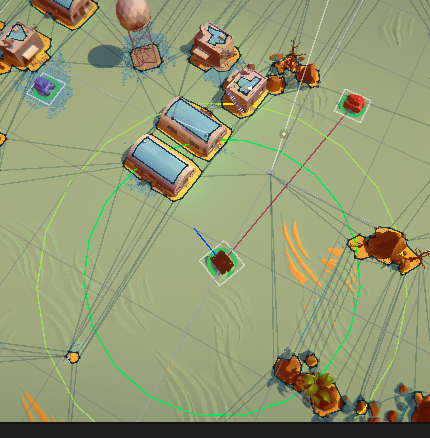
\includegraphics[width=0.5\textwidth]{imgs/tankai.png}
        \caption{The new enemy tank.}
        \label{fig:tankai}
    \end{figure}

\section{Exercise 2: Adjust the Camera}
    I added the new aiTank array to the previous existing targets array, then combined them.

    \begin{minted}{csharp}
        private void SetCameraTargets()
        {
            // Create a collection of transforms the same size as the number of tanks and AI tanks combined.
            Transform[] targets = new Transform[m_Tanks.Length + aiTanks.Length];


            for (int i = 0; i < m_Tanks.Length; i++)
            {
                // ... set it to the appropriate tank transform.
                targets[i] = m_Tanks[i].m_Instance.transform;
            }

            // Add AI tanks to the targets array.
            for (int i = 0; i < aiTanks.Length; i++)
            {
                targets[m_Tanks.Length + i] = aiTanks[i].m_Instance.transform;
            }

            m_CameraControl.m_Targets = targets;
        }
    \end{minted}

\section{Exercise 3: Point and Shoot}
    As seen in Figure \ref{fig:tankai}, the tank will follow the nearest player tank, and then get closer after the green circle touches the player. Then it will fire a shot every 2 seconds.


\end{document}